    In this module, we calculate the similarity measure of the solutions with each other which is then later used for clustering.
    
    The central idea is to generate \textit{Program Dependence Graphs} \cite{PDG} for the solutions and check for sub-graph isomorphism between any two PDG's. If it is sub-graph isomorphic then based on the number of vertices mapped we calculate similarity. (No. of mapped vertices of Graph G1 / Total no. of vertices of Graph G2) [G1 sub-graph isomorphic to G2]

    PDG's are generated for each function. In this instance we assume that the datset contains only one function(main) and genearte PDG's for main functions. % A solution can have multiple functions with different function names for each of the solution. So to map PDG's properly, we generate a function call for the solution and do a simple linear mapping based on the positions of the function calls in the stack.Function call can be generated using the \textit{cflow} command in \textit{Linux}.
    
    We use \textit{frama-c} software to generate PDG's of the solution. This creates a DOT file for each of the function. To parse this, we use a DOT parser in python to get a grpah with vertices and nodes.We use $\gamma$-isomorphism method to calculate similarity. This$\gamma$-isomorphism method checks for sub-graph isomorphism between the PDG's and calculates similarity as mentioned above.  
    
\textit{Summary:}
\begin{itemize}
    \item Create PDG's using frama-c for each solution.
        \begin{itemize}
            \item DOT files for each function
            \item \textit{frama-c -pdg -pdg-dot filename c-programfile }.
        \end{itemize}
    \item Extract graph nodes and edges from DOT file using a DOT parser in python
    \item Calculate similarity measure using $\gamma$-isomorphism as mentioned above.
\end{itemize}

Output of this module is similarity measure of each pairs of solution ranging from $0$ to $1$ with $1$ being high similarity and 0 being no similarity.

\subsubsection{Implementation Details:}
    \begin{itemize}
        \item For each program, PDG has to be generated, we use \textit{frama-c} to generate a DOT file which contains the PDG.
        \item A DOTParser for python was used to extract nodes and edges from the DOT file. This was converted to a NetworkX graph in python.
        \item Sub graph isomorphism algorithm was used to calculate similarity.
    \end{itemize}
    
    \paragraph{Program Dependence Graph}
        
        \textit{Frama-c} is a set of interoperable program analyzers for C programs. We use \textit{Frama-c} to generate dependency graph in the form of DOT files for C programs. While it generates for most of the C programs it does not encompass the entire C language. 
        
        Frama-c (Flourine version) the stable release for Ubuntu 14.04 does not work with Variable Length array, the latest release of Frama-c (Phosphorous) while it works with single dimensional variable length array it doesnot for multi-dimensional arrays.
        
        The output of Frama-c's pdg generation is a DOT file which contains the nodes and edges of the PDG. DOT files are hard to interpret and contains unnecessary details, so a DOTParser was used to get only the nodes and edges. This was then used to instantiate a NetworkX graph (a python library for graphs) which was selected for it's vast graph related library.
        
    \paragraph{$\gamma$-isomorphism}
        
        We follow the algorithm provided in \cite{GPLAG} named $\gamma$-isomorphism as it uses a $\gamma$-filtering technique to eliminate certain graphs before performing subgraph isomorphism.
        
        Sub graph Isomorphism is an NP-Complete problem which means that there is no polynomial time solution. (Note that Graph Isomorphism is neither P nor NP-complete but it's generalisation(sub-graph isomorphism) is NP-complete). Over the years there have been many heuristic solutions that attempt to solve this for a specific set of graphs like the Glasgow algorithm \cite{Glasgow}, the VF2 algorithm \cite{VF} and recently the LAD filtering algorithm \cite{pathLAD}.
        
        Initially the \textit{VF2} algorithm was implemented as it was used in the algorithm mentioned in \cite{GPLAG}, we found that the algorithm is very time-consuming, while for graphs with very less nodes (in the range of 20 to 30) it calculates in seconds, the higher the vertex count (usually in the range of 100's which is the case for our dataset) it sometimes takes days to calculate!!
        
        Due to this the \textit{VF2} algorithm approach was abandoned and the latest development in sub graph isomorphism the LAD filtering approach was chosen. The latest variant, \textit{pathLAD} \cite{pathLAD}, was used. A time limit was set which can act as a threshold as to when the search can be discontinued.
        
        While the LAD algorithm works much faster than \textit{VF2}, there are still cases where sub-graphs could not be found within the time-limit. In some cases increasing the time-limit by a few seconds leads to solutions where it would not have found in the decreased time-space. This leads to drastic change in the output of the next phase.
        
\subsubsection{Suggestion:}
    Due to the unreliability of sub graph-isomorphism, find other similarity metrics like LOC, Function count, running time, memory usage, $\cdots$. Use a weighted average of these metrics to calculate a similarity index. This will lead to less dependence on graph isomorphism which will not drastically alter the overall output.

        \begin{figure}[H]
            \centering
                \centering
                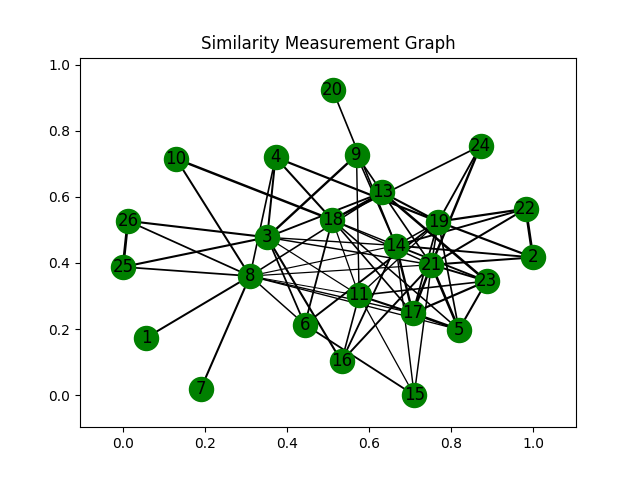
\includegraphics[height=1.2in]{Images/similarity_ensemble_1.png}
                \caption{Similarity Measure Ouput}
        \end{figure}